\section{Results}

This section presents the empirical results of the study. First, the
classification performance of the investigated models and the results of the
H1 test are reported. This is followed by the results of the SHAP-based
explainability analysis and the test of H2.

\subsection{Classification Performance and Model Selection}

The classification performance of the investigated models was evaluated on
the previously separated hold-out dataset comprising 5,709 tickets. Macro-F1
($F1_{\mathrm{macro}}$) was used as the primary performance measure.
Macro-Precision ($P_{\mathrm{macro}}$), Macro-Recall
($R_{\mathrm{macro}}$), and Accuracy (Acc) are reported as complementary
metrics. For the cross-model comparison, FS4 was selected as the common
feature basis based on the cross-validation results. With a Macro-F1 of
0.5123 averaged across all seven classifiers, FS4 achieved the highest mean
cross-validation performance. Table~\ref{tab:holdout_performance} summarizes
the hold-out results of the seven classifiers on FS4 and of the finally
selected FS5-LightGBM model.

\begin{table}[ht]
    \centering
    \caption{Classification performance of the seven classifiers on the common
    feature set FS4 and of the final FS5-LightGBM model on the hold-out dataset.}
    \label{tab:holdout_performance}
    \begin{tabular}{llrrrr}
        \toprule
        Feature set & Classifier & $F1_{\mathrm{macro}}$ &
        $P_{\mathrm{macro}}$ & $R_{\mathrm{macro}}$ & Acc \\
        \midrule
        FS4 & Logistic Regression    & 0.5397 & 0.5379 & 0.5422 & 0.5568 \\
        FS4 & Linear SVM             & 0.5406 & 0.5414 & 0.5405 & 0.5616 \\
        FS4 & Complement Naive Bayes & 0.4893 & 0.4888 & 0.4936 & 0.5129 \\
        FS4 & kNN                    & 0.5478 & 0.5766 & 0.5396 & 0.5733 \\
        FS4 & Random Forest          & 0.5566 & 0.5929 & 0.5493 & 0.5936 \\
        FS4 & XGBoost                & 0.5112 & 0.5696 & 0.5083 & 0.5617 \\
        FS4 & LightGBM               & 0.5594 & 0.5910 & 0.5522 & 0.5950 \\
        FS5 & LightGBM               & 0.5597 & 0.5903 & 0.5527 & 0.5952 \\
        \bottomrule
    \end{tabular}
\end{table}

Within the FS4 comparison, LightGBM achieved the highest classification
performance, with a Macro-F1 of 0.5594. The lowest Macro-F1 was observed for
Complement Naive Bayes, with a value of 0.4893.

To test H1, each of the six alternative classifiers on FS4 was compared
pairwise with the Logistic Regression baseline. The effect size was calculated
according to Equation~\ref{eq:h1_delta}. The observed differences and their
corresponding 95\% confidence intervals are shown in the pairwise comparison
with the Logistic Regression baseline (see Figure~\ref{fig:h1_pairwise}).

\begin{figure}[ht]
\centering
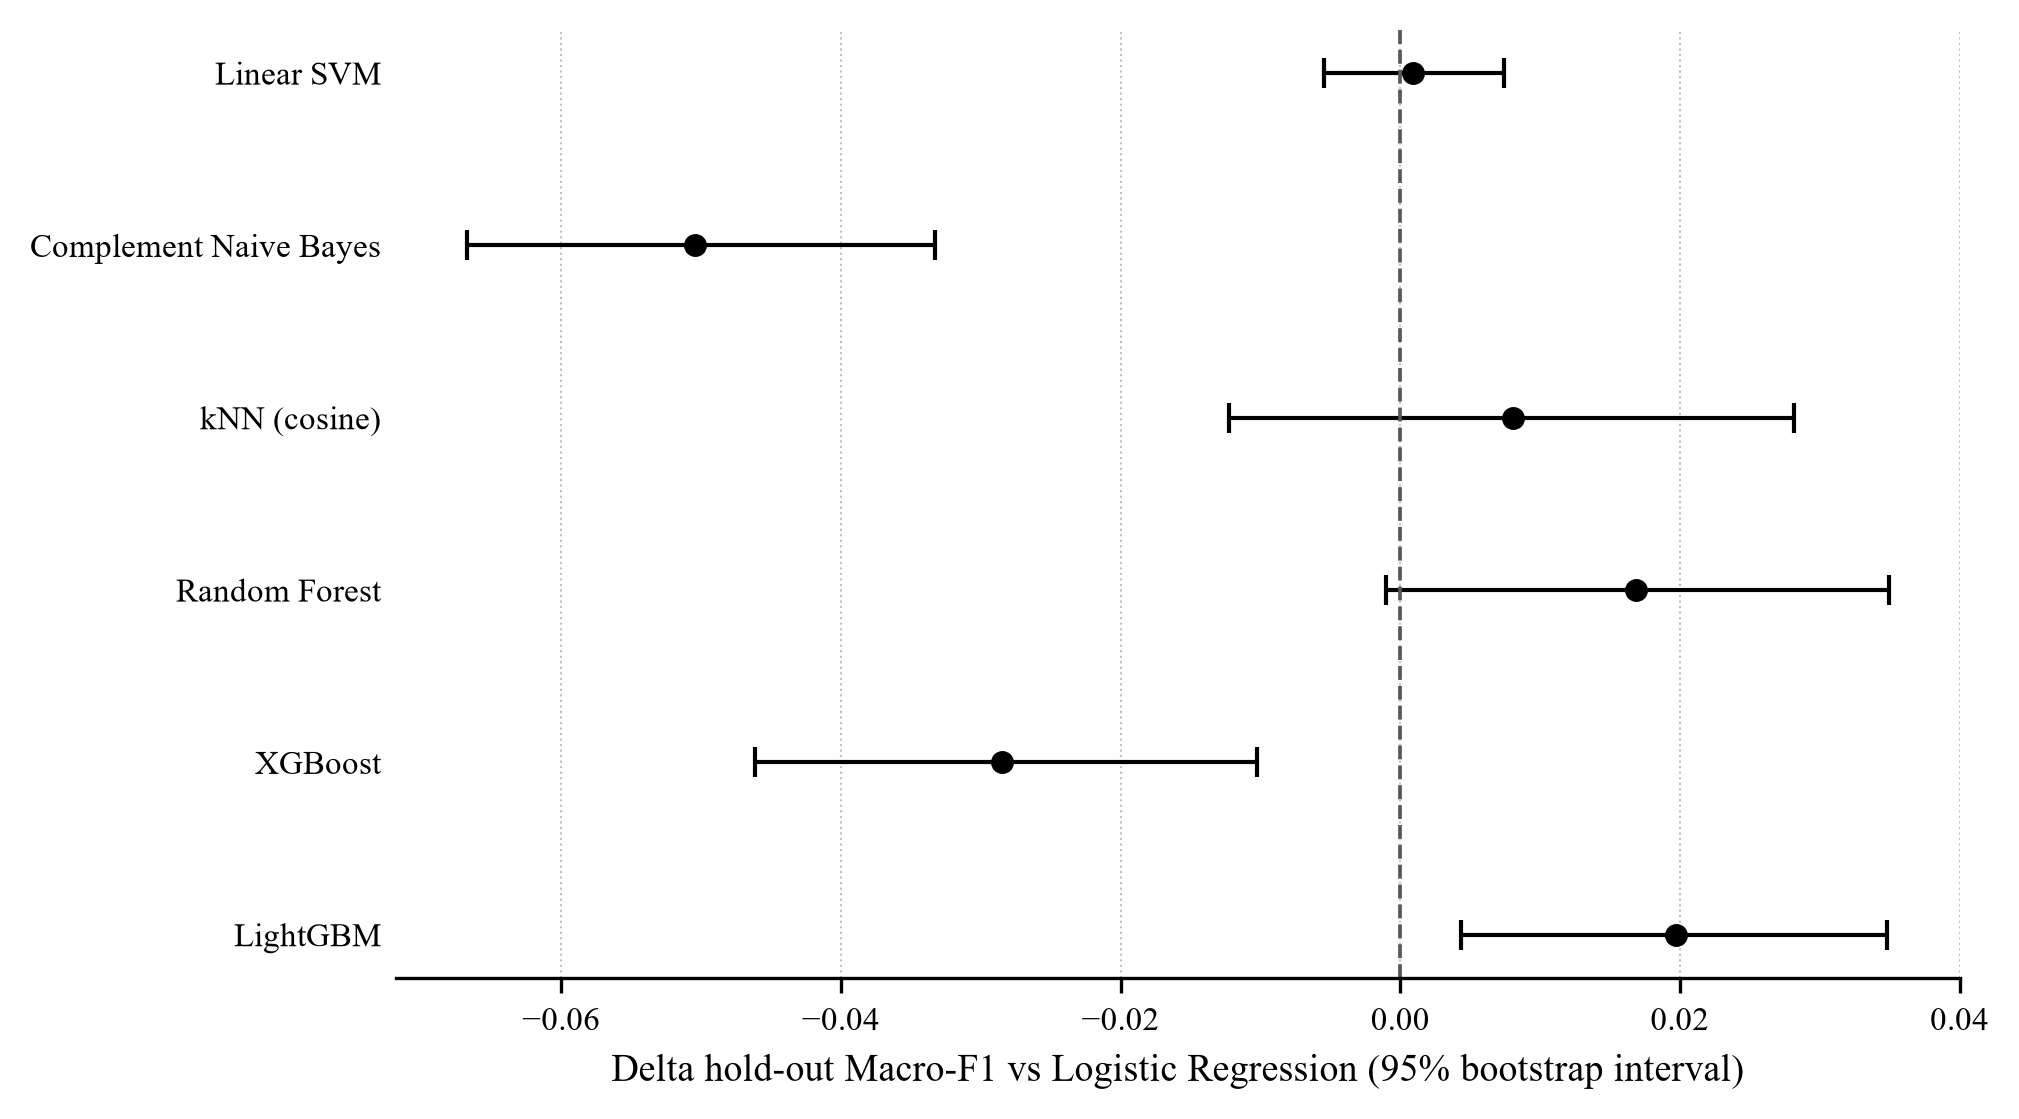
\includegraphics[width=\linewidth]{figures/04_H1_pairwise_macro_f1_differences.png}
\caption{Pairwise differences in Macro-F1 between the alternative classifiers
and the Logistic Regression baseline on FS4.}
\Description{Forest plot comparing six alternative classifiers with Logistic
Regression on FS4. LightGBM has a positive confidence interval entirely above
zero. Random Forest and kNN have positive point estimates with intervals
crossing zero, Linear SVM is close to zero, and XGBoost and Complement Naive
Bayes show negative differences.}
\label{fig:h1_pairwise}
\end{figure}

For LightGBM, a positive difference of
$\Delta F1_{\mathrm{macro}} = 0.0197$ was obtained. The 95\% confidence
interval was entirely above zero, 95\% CI [0.0044, 0.0348], and the
directional comparison remained statistically significant after Holm
correction for multiple testing ($p_{\mathrm{Holm}} = 0.024$).

A positive difference was also observed for Random Forest
($\Delta F1_{\mathrm{macro}} = 0.0169$), although the 95\% CI
[$-0.0010$, 0.0350] included zero, and the difference was not statistically
significant after Holm correction ($p_{\mathrm{Holm}} = 0.161$). No
statistically significant improvements over the baseline were found for kNN
($\Delta F1_{\mathrm{macro}} = 0.0081$, 95\% CI [$-0.0122$, 0.0282],
$p_{\mathrm{Holm}} = 0.855$) or Linear SVM
($\Delta F1_{\mathrm{macro}} = 0.0009$, 95\% CI [$-0.0054$, 0.0074],
$p_{\mathrm{Holm}} = 1.000$). For XGBoost
($\Delta F1_{\mathrm{macro}} = -0.0285$, 95\% CI
[$-0.0462$, $-0.0103$]) and Complement Naive Bayes
($\Delta F1_{\mathrm{macro}} = -0.0504$, 95\% CI
[$-0.0668$, $-0.0333$]), the observed effects were entirely in the opposite
direction.

Since at least one of the six prespecified comparisons showed a positive
effect that remained statistically significant after Holm correction, H1 is
supported.

The final model selected based on cross-validation was LightGBM with feature
set FS5. It achieved a mean cross-validation Macro-F1 of 0.5330
(SD = 0.0097) and a Macro-F1 of 0.5597 on the separate hold-out dataset
(95\% CI [0.5431, 0.5757]).

At the class level, the final FS5-LightGBM model achieved a Precision of
0.6457, a Recall of 0.6819, and an F1 score of 0.6633 for high-priority
tickets. For the medium-priority class, Precision was 0.5577, Recall was
0.6471, and F1 was 0.5991. The lowest class-specific performance was observed
for low-priority tickets, with a Precision of 0.5674, a Recall of 0.3291, and
an F1 score of 0.4166. Low-priority tickets were most frequently confused with the medium-priority class, whereas medium- and high-priority tickets were classified correctly more often. The corresponding class-specific prediction pattern is
shown in the normalized confusion matrix (see Figure~\ref{fig:final_confusion_matrix}). 

\begin{figure}[ht]
\centering
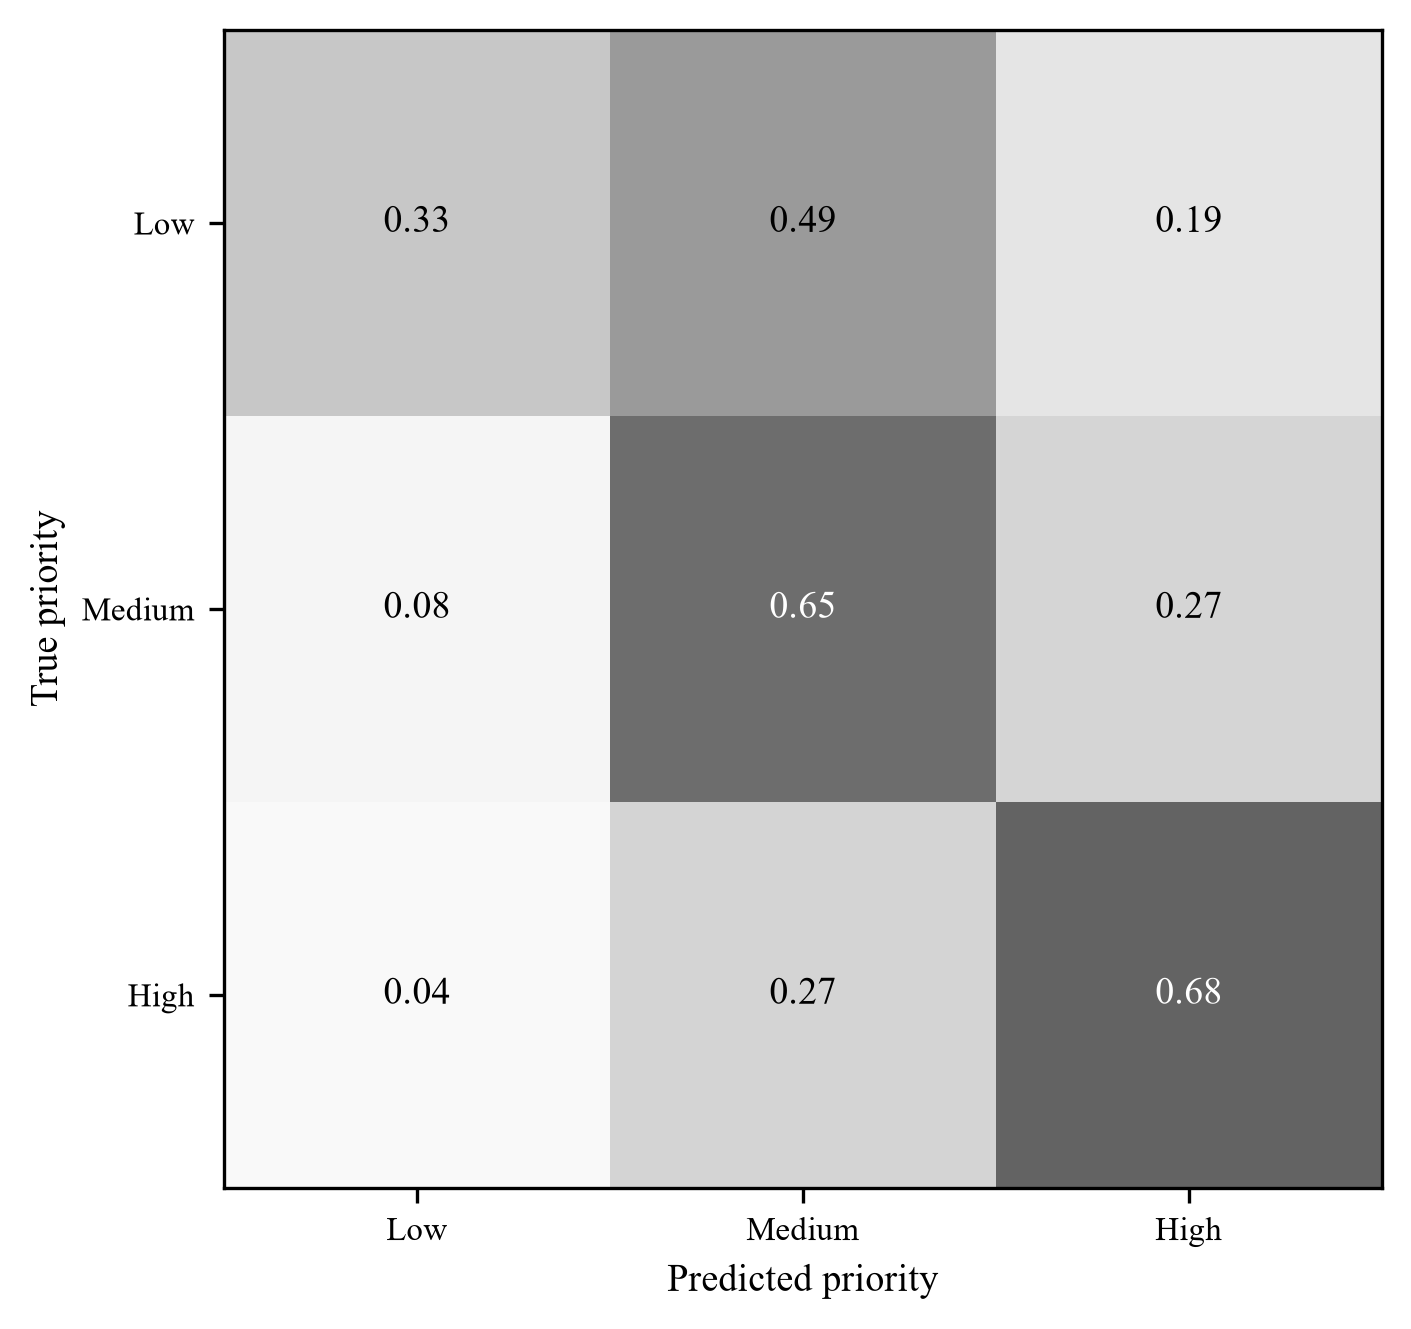
\includegraphics[width=0.72\linewidth]{figures/04_final_model_confusion_matrix.png}
\caption{Normalized confusion matrix of the final FS5-LightGBM model on the
hold-out dataset.}
\Description{Three-by-three row-normalized confusion matrix. Low-priority
tickets are predicted as low, medium, and high with proportions 0.33, 0.49,
and 0.19. The corresponding proportions are 0.08, 0.65, and 0.27 for
medium-priority tickets and 0.04, 0.27, and 0.68 for high-priority tickets.}
\label{fig:final_confusion_matrix}
\end{figure}

\subsection{SHAP-Based Explainability and Attribution Patterns}

The SHAP-based explanation compactness of the seven classifiers was examined
on the common feature set FS4 based on the concentration of absolute SHAP
attributions. The primary measure was Top-10 concentration, defined as the
proportion of the total absolute SHAP mass attributable to the ten features
with the highest absolute attributions. Higher values correspond to a stronger
concentration of the attributions on a small number of features. Figure~\ref{fig:h2_compactness} shows the Top-10 concentration of absolute SHAP mass across the
common explainability sample.

\begin{figure}[ht]
\centering
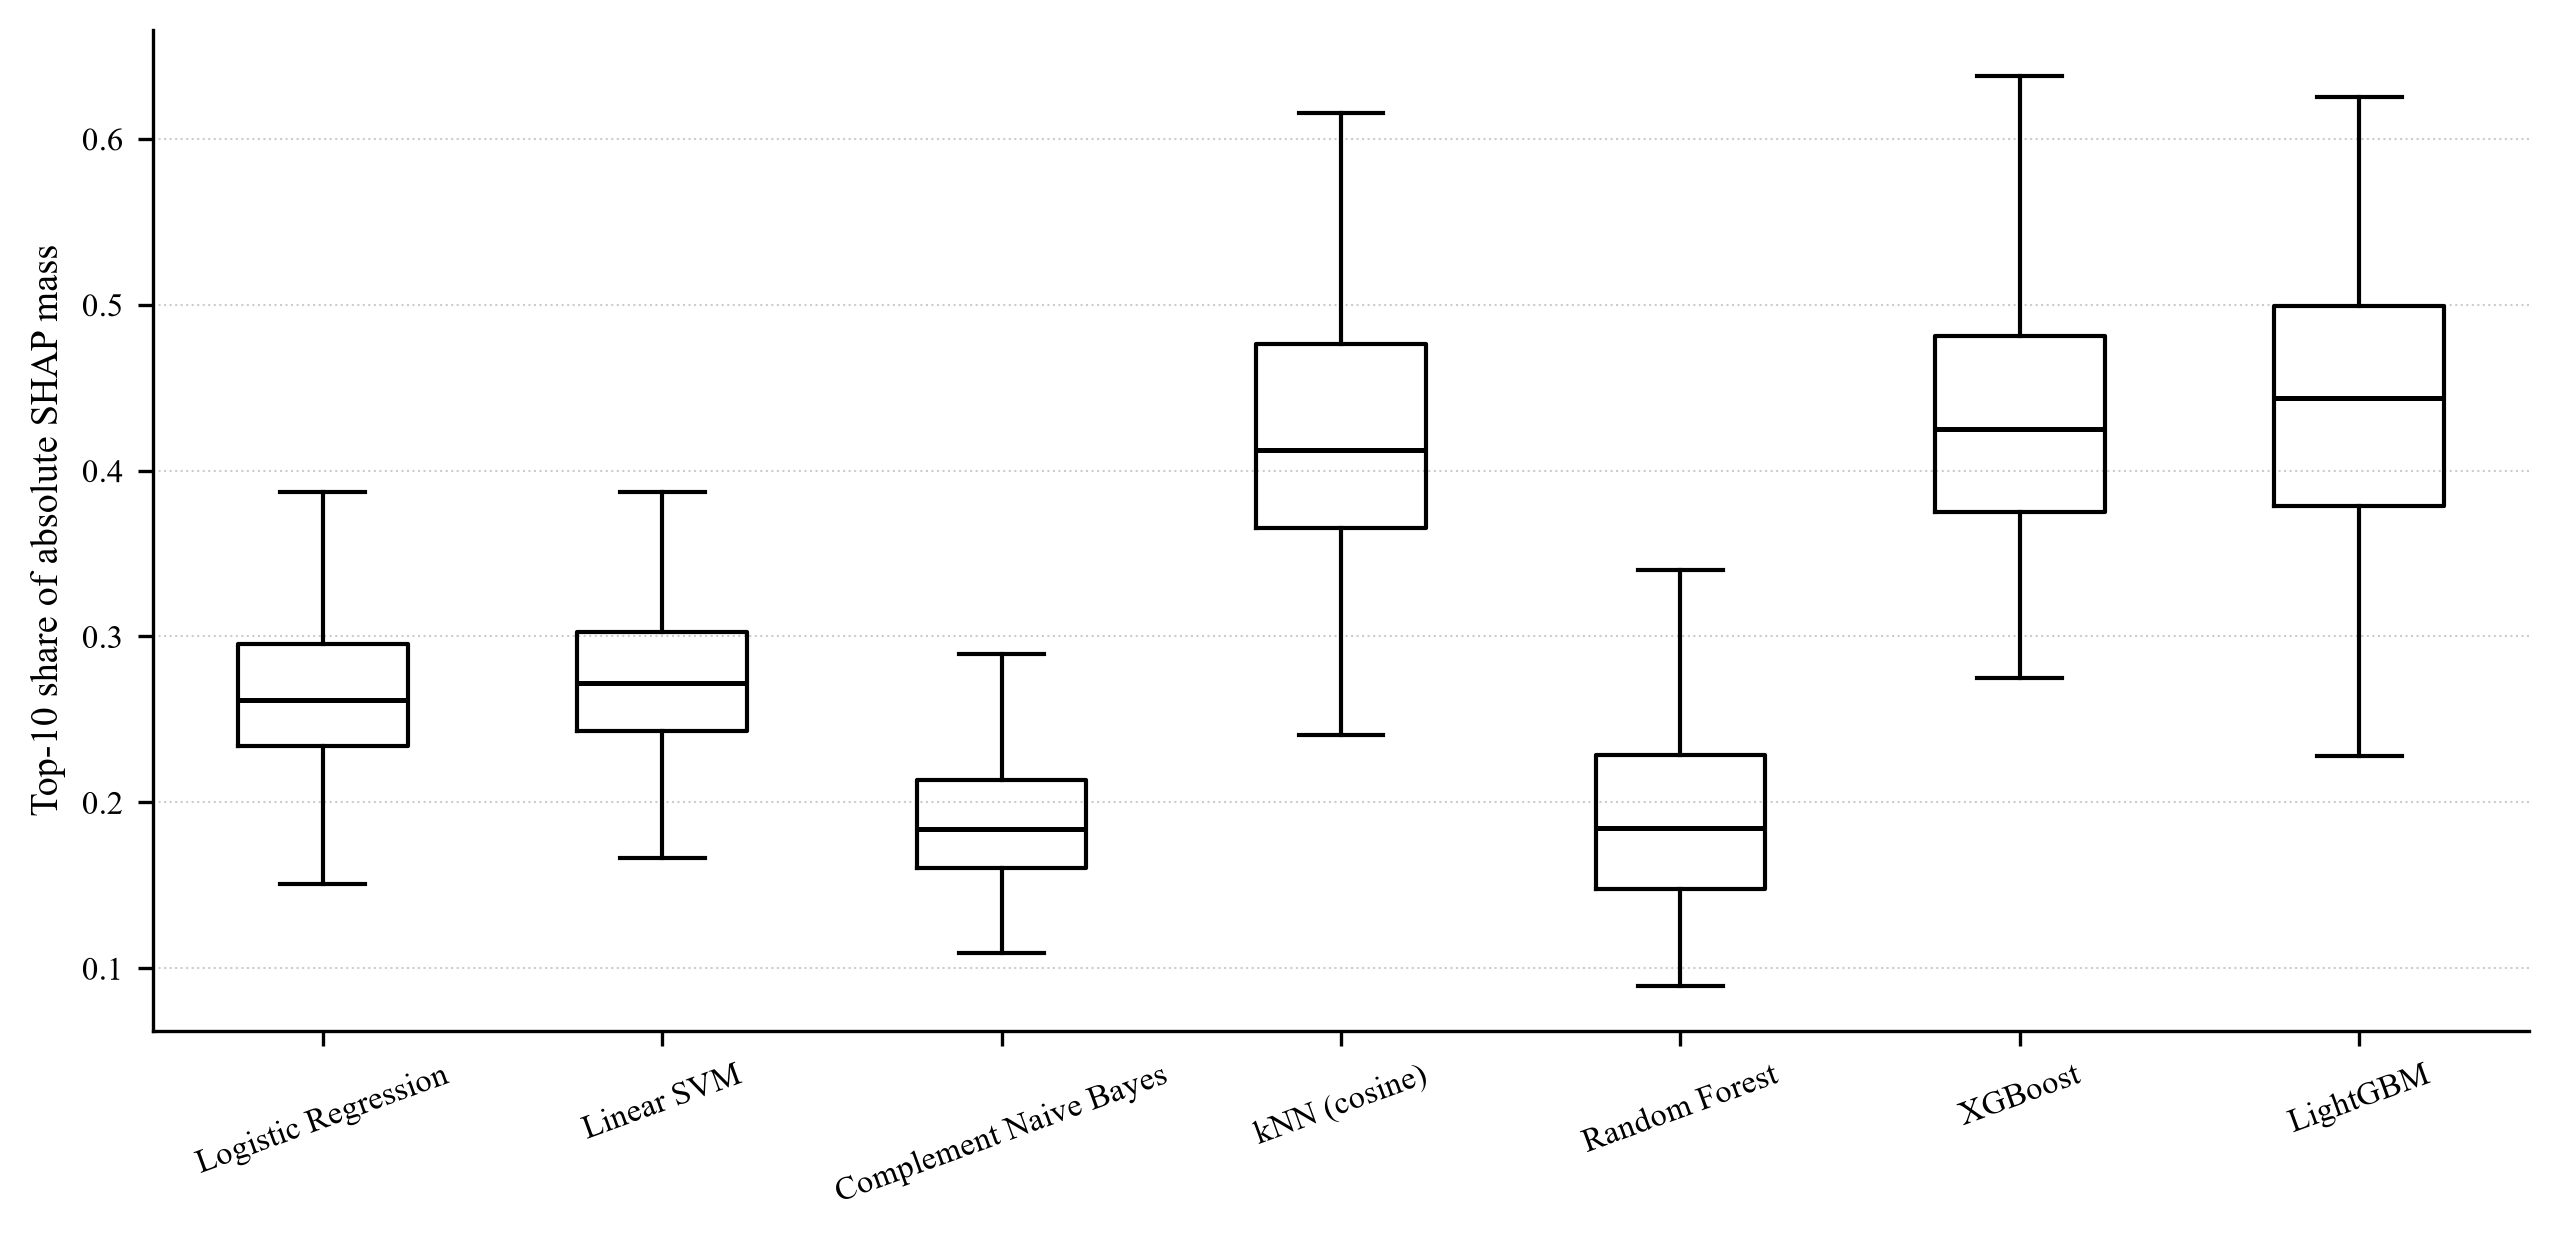
\includegraphics[width=\linewidth]{figures/05_h2_compactness_by_model.png}
\caption{SHAP-based explanation compactness of the seven classifiers on FS4.}
\Description{Boxplots of Top-10 absolute SHAP-mass concentration for the seven
classifiers. Complement Naive Bayes and Random Forest show the lowest
concentrations, Logistic Regression and Linear SVM intermediate values, and
kNN, XGBoost, and LightGBM substantially higher concentrations.}
\label{fig:h2_compactness}
\end{figure}

The mean Top-10 concentration was 0.2657 for Logistic Regression and 0.2740
for Linear SVM. Lower values were observed for Complement Naive Bayes
(0.1882) and Random Forest (0.1916). Higher concentrations were obtained for
kNN (0.4238), XGBoost (0.4286), and LightGBM (0.4388).

To test H2, the pairwise differences in Top-10 concentration were calculated
according to Equation~\ref{eq:h2_delta}. Positive values indicate higher
explanation compactness for Logistic Regression. For Complement Naive Bayes,
the difference was $\Delta \mathrm{Top10} = 0.0775$. The 95\% CI
[0.0727, 0.0823] was entirely above zero, and the Holm-corrected directional
test was statistically significant ($p_{\mathrm{Holm}} < 0.001$). Logistic
Regression also showed a significantly higher Top-10 concentration than
Random Forest ($\Delta \mathrm{Top10} = 0.0741$, 95\% CI
[0.0676, 0.0805], $p_{\mathrm{Holm}} < 0.001$).

For Linear SVM, in contrast, the difference was
$\Delta \mathrm{Top10} = -0.0083$, 95\% CI
[$-0.0106$, $-0.0062$]. The confidence intervals were also entirely below
zero for kNN ($\Delta \mathrm{Top10} = -0.1582$, 95\% CI
[$-0.1670$, $-0.1489$]), XGBoost
($\Delta \mathrm{Top10} = -0.1630$, 95\% CI
[$-0.1700$, $-0.1558$]), and LightGBM
($\Delta \mathrm{Top10} = -0.1731$, 95\% CI
[$-0.1831$, $-0.1632$]). The directional comparisons were not statistically
significant in these cases.

Since at least one of the six prespecified comparisons showed a positive
effect that remained statistically significant after Holm correction, H2 is
supported. This criterion was met for Complement Naive Bayes and Random
Forest. At the same time, the results show that Logistic Regression did not
exhibit higher explanation compactness than all investigated classifiers.

The robustness analyses confirmed the H2 pattern for Complement Naive Bayes
across all five investigated operationalizations. For Random Forest, the
advantage of Logistic Regression was observed for Top-5 concentration,
Top-20 concentration, and Top-10 concentration restricted to active features,
but not for \(K_{80}\) or normalized entropy. The result for Random Forest was
therefore dependent on the measure used.

The complementary faithfulness analysis showed that removing the ten active
text features with the highest absolute SHAP values resulted in a larger
decrease in the score of the originally predicted class than removing the same
number of randomly selected active text features in more than half of the
cases for all seven classifiers. The corresponding proportion ranged from
60.67\% for XGBoost to 98.67\% for Complement Naive Bayes. For Logistic
Regression, the proportion was 82.67\%, compared with 72.00\% for LightGBM.
For XGBoost, the comparison between approximate and exact SHAP contributions
yielded a high rank correlation.

The class-switch rate was also higher for all seven classifiers after removal
of the ten most important SHAP text features than after removal of randomly
selected active text features. Following SHAP-based removal, class-switch
rates ranged from 0.1600 to 0.4200, compared with 0.0400 to 0.1173 following
random removal.

In addition, the finally selected FS5-LightGBM model was analyzed separately
using SHAP. With respect to the predicted class in each case, 82.33\% of the
total absolute SHAP mass was attributable to text features and 15.63\% to the
ticket queue. Ticket type accounted for 1.10\%, sentiment features for
0.94\%, and language for less than 0.01\%. At the class level, the proportion
attributable to text features was 80.17\% for low priority, 90.23\% for
medium priority, and 75.34\% for high priority. The corresponding proportions
attributable to the queue were 18.56\%, 8.95\%, and 20.92\%.

The qualitative plausibility assessment of the twelve local comparison cases
yielded a heterogeneous picture. While some of the SHAP explanations were
considered plausible in terms of their content, others were rated as only
partially plausible or not plausible, particularly when the attributions were
dominated by features with limited discriminative value or features that were
difficult to interpret.